%!TEX root = ../report.tex

\section{Stereovision} % (fold)
\label{sec:stereopsis}

\subsection{Introduction}
In this section, the solution adopted for the location of the target in the 3D space through the vision system, the reasons that led to this approach, the assumptions made and the obtained results are presented. 
A more detailed explanation of the 2D image processing performed for the target tracking can be found in \ref{sec:feature_extraction}.

\subsection{Stereopsis}
Due to the fact that two vision systems were available on the setup, the first step was to decide which one to employ and the method to compute disparity. 
After a slight evaluation of resources the chosen one was the stereo rig, utilized to carry out sparse stereo with a single well-defined point. 
Thus, the next points contain the steps to compute the position of a point in 3-space given its image in two views and the camera matrices. 

Through the acquired pairs of images, the pixel coordinates of the center of gravity of the target are extracted by the algorithm presented in \ref{sec:feature_extraction} and they are used to calculate its 3D coordinates referred to the camera reference frame by means of linear triangulation methods.

\subsection{Camera model}
As a consequence of the need of a defined relation between the image and the object space, the cameras must be used as a mapping. 
The mathematical model assumed for the camera is the basic pinhole structure, described in ***(Hartley et al). 
This model defines a linear projection from the 3D world to the image plane, and contains the intrinsic parameters that relates the camera and the image reference frames as showed in equation \ref{eq:pinhole_model}. 

\begin{equation}
x = K·A·X
\label{eq:pinhole_model}
\end{equation}  

***** Define the equation members

Since the linearity assumed by this model does not hold due to imperfections in the lens, a distortion model needs to be added to the calculations. The Plumb Bob distortion model, introduced in ***(Brown) is applied here since it is the one used by ROS.

\subsection{Calibration}
In order to obtain the intrinsic parameters for the camera model, a stereo calibration process based on the technique presented in ***(Zhang) has been carried out for both Bumblebee2 1394a cameras by means of a ROS node. 
The node just needs to be provided enough images of a 2D calibration pattern in different positions. It computes the projection of the points on the pattern and solves the resulting equations system in a least squares fashion as described in ****reference(). The output of the node are the camera and projection matrices of the cameras, the set of parameters for the distortion model and the homography for the image rectification. 

\subsection{Triangulation}
At this point the algorithm yields the camera matrices and the image point correspondences {xi, xi'}.
The next step is to define a suitable triangulation method light but robust enough to be executed in live with sufficient accuracy, since the whole system will rely on this task. 

Due to the acquisition errors in the measured image coordinates, a simple approach based on back-propagation of rays from the image points is very unlikely to succeed. This is because in most of the cases the rays will not intersect in the 3D point. 

\begin{figure}[h]
    \centering
    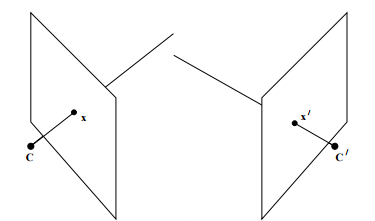
\includegraphics[width=0.8\textwidth]{images/Back-Projection}
    \caption{Back-Projection rays error}
    \label{fig:Back-Projection}
\end{figure}


% section stereopsis (end)